\documentclass[12pt,a4paper,italian,twoside, openany]{book}

% Set up data, if you need to add a package, go here
%
\usepackage[utf8]{inputenc}
\usepackage[T1]{fontenc}
\usepackage{graphicx}
\usepackage[nottoc]{tocbibind}
\usepackage{booktabs}
\usepackage[margin=1.5in]{geometry}
\usepackage[italian]{babel}
\usepackage{algorithm}
%\usepackage{arevmath}     % For math symbols
\usepackage[noend]{algpseudocode}
\usepackage{multirow}
\usepackage{mathtools}
\usepackage[normalem]{ulem}
\useunder{\uline}{\ul}{}
\usepackage{wrapfig}
\usepackage{todonotes}
\usepackage{adjustbox}
%\usepackage{fixltx2e}
\usepackage{caption}
\usepackage{subcaption}
\usepackage{array}
\usepackage{mathtools}
\usepackage[hidelinks]{hyperref}

\hypersetup{}
\newcolumntype{P}[1]{>{\centering\arraybackslash}p{#1}}

\usepackage[square,numbers]{natbib}
\makeatletter
\renewcommand\bibsection%
{
  \section*{\refname
    \@mkboth{\MakeUppercase{\refname}}{\MakeUppercase{\refname}}}
}
\makeatother
%%%%%%

\usepackage{xcolor}

\definecolor{codegreen}{rgb}{0,0.6,0}
\definecolor{codegray}{rgb}{0.5,0.5,0.5}
\definecolor{codepurple}{rgb}{0.58,0,0.82}
\definecolor{backcolour}{rgb}{0.95,0.95,0.92}



% macro
\newcommand{\matchNews}[1]{\emph{$news\_match$}\textsubscript{\texttt{\lowercase{#1}}}}
\newcommand{\matchRatio}[1]{\emph{$match\_ratio_{#1}$}}

\begin{document}

% viene caricato il logo vettoriale UFFICIALE dell'università
%\begin{spacing}{0.90}
\begin{center}
    {\Large \thispagestyle{empty}}{
\includegraphics[scale=0.1]{images/logo.png}}\par
\end{center}
%\end{spacing}

\noindent 
\begin{center}
    \textbf{\Large Università degli Studi di Cagliari}%\par
\end{center}%{\LARGE \par}
\vspace{-1em}
\noindent 
\begin{center}
    \textbf{\large Facoltà di Scienze}\par
\end{center}{\large \par}
\vspace{-1em}
\noindent
\begin{center}
    {\large Corso di Laurea Triennale in Informatica}\par
\end{center}{\large \par}

\vspace{7em}

\noindent
\begin{center}
    \textbf{\Large Misura di posizione e velocità}\par
    \vspace{0.6em}
    \textbf{\Large in sistemi di sorveglianza stradale}\par
\end{center}{\LARGE \par}

%\begin{spacing}{0.90}
\vspace{4cm}
\textbf{\large Relatore:}{\large \hfill{}}\textbf{\large Candidato:}{\large \par}
%\end{spacing}

{\large Prof. Salvatore M. Carta\hfill{}Nicola Sansoni~}{\large \par}
\vspace{1cm}
\textbf{\large Co-Relatore:}{\large \par}
{\large Dott. Alessandro Sebastian Podda}

\vspace{2cm}

\begin{center}
    {\large ACADEMIC YEAR 2020/2021}{\large \par}
\end{center}


% ----------------------------- ABSTRACT ------------------------------------
\setlength{\parskip}{\bigskipamount}
\renewcommand{\baselinestretch}{1.4}\normalsize
\chapter*{Abstract}
Nelle città di oggi sono sempre più diffusi sistemi di sorveglianza a camera fissa.
Tali sistemi consentono di monitorare il traffico cittadino, rendendo le città più sicure.
Grazie al progresso degli ultimi anni nei campi di Machine Learning e Object Detection, è possibile rilevare in tempo reale entità, come veicoli e persone, inquadrati da tali camere.
Risulta quindi di interesse estrarre informazioni accurate riguardo alla posizione e alla velocità di tali entità. 
Tali informazioni possono essere utilizzate in tempo reale nella fase di tracciamento delle entità, e nello sviluppo di euristiche per il rilevamento di anomalie.
Queste anomalie possono essere notificate alle autorità in modo da ridurre i tempi di risposta in presenza di situazioni di rischio.
Possono anche essere utilizzate in un secondo tempo per studiare e modellare il comportamento delle entità, così da sviluppare interventi che aumentino la sicurezza delle aree monitorate.

Le informazioni estratte dall'immagine presentano però distorsioni dovute alla prospettiva della camera e errori legati alla precisione dell'Object Detection.
Questa tesi descrive un possibile approccio per la correzione della distorsione proiettiva e del errore legato all'Object Detection, permettendo l'acquisizione di misure accurate relative a posizione e velocità delle entità inquadrate.


% ------------------------------- INDICE ---------------------------------------
\renewcommand{\baselinestretch}{1}\normalsize


\frontmatter 						% numerazione romana
\tableofcontents

\pagestyle{plain}
%\makeheadrule{headings}{\textwidth}{0.3pt}

\renewcommand{\baselinestretch}{1.4}\normalsize

\mainmatter
\chapter{Introduzione e stato dell'arte}
\label{sec:introduzione}

% Homogenous matrix: 4 points, automatic generation; Single view metrology.
% Kalman filters, EWMA, Moving averages

\section{Contesto e motivazioni}

Lo sviluppo di un sistema di rilevazione di anomalie stradali richiede la conoscenza dei dati relativi alle entità presenti nella scena inquadrata dalla telecamera di sorveglianza.
In particolare risultano necessari i dati relativi a posizione, velocità e categoria delle entità.
La categoria è importante per differenziare persone, veicoli e oggetti, posizione e velocità sono importanti per comprendere come questi si comportano e interagiscono.
Possiamo ottenere la categoria delle entità e la loro posizione nell'immagine utilizzando una \emph{CNN}.
\textbf{TODO: DUE PAROLE SUL TRACKING}

Sia posizione che velocità ottenute in questo modo sono in spazio immagine e non corrispondono con le misure reali.
Inoltre entrambe presentano errori simili a rumore, derivati dalla precisione non perfetta dell'Object Detection.

Per ottenere un sistema affidabile è necessario correggere in modo efficace sia la distorsione prospettica sia il rumore.

\section{Obiettivo della tesi}
\begin{itemize}
	\item Indicare una metodologia per la correzione della distorsione prospettica per inquadrature con orientamento arbitrario da applicare al contesto stradale.
	\item Indicare una metodologia per la correzione del rumore delle misure di posizione e velocità per entità come persone e veicoli.
\end{itemize}

\section{Attività della tesi}

\begin{itemize}
	\item Studio delle trasformazioni di proiezione
	\item Studio delle tecniche di correzione del rumore
	\item \textbf{TODO: il resto}
	\item Confronto tra risultati con e senza correzione
\end{itemize}

\section{Schema della tesi}

Nel capitolo \ref{sec:funzionalita} sono illustrati in dettaglio i problemi affrontati e il modo in cui sono affrontati allo stato dell'arte.
Nel capitolo \ref{sec:architettura} è illustrata l'architettura del sistema di rilevazione di anomalie stradali.
Nel capitolo \ref{sec:prospettiva} è descritta la soluzione scelta per la correzione della distorsione prospettiva, la sua implementazione e le problematiche riscontrate.
Nel capitolo \ref{sec:rumore} è descritta la soluzione scelta per la correzione del rumore presente nelle misurazioni, la sua implementazione e le problematiche riscontrate.
Infine nel capitolo \ref{sec:conclusioni} è riassunto il lavoro svolto, sono discussi i risultati ottenuti e sono suggeriti possibili sviluppi e miglioramenti.

\chapter{Studio del problema}
\label{sec:teoria}

%rivedere tutto il paragrafo
Un'immagine è una rappresentazione dello spazio reale generata da una camera.
La camera genera l'immagine utilizzando un sensore per ``catturare'' la luce proveniente dallo spazio reale. 
Possiamo ragionevolmente considerare la luce come dei raggi perfettamente lineari che si muovono a velocità infinita, e possiamo immaginare il sensore come la porzione di un piano bidimensionale in cui ogni punto cattura un raggio di luce.
Modelliamo in questa tesi la nostra camera come una \emph{camera oscura} (figura \ref{fig:camera oscura}).
Una \emph{camera oscura} è composta da una ``scatola'' con una singola apertura puntiforme attraverso il quale la luce può passare.
Questo ci permette di ignorare le distorsioni causate dalla lente della camera.
\begin{figure}
    \caption{Camera oscura}
    \label{fig:camera oscura}
    \centering
    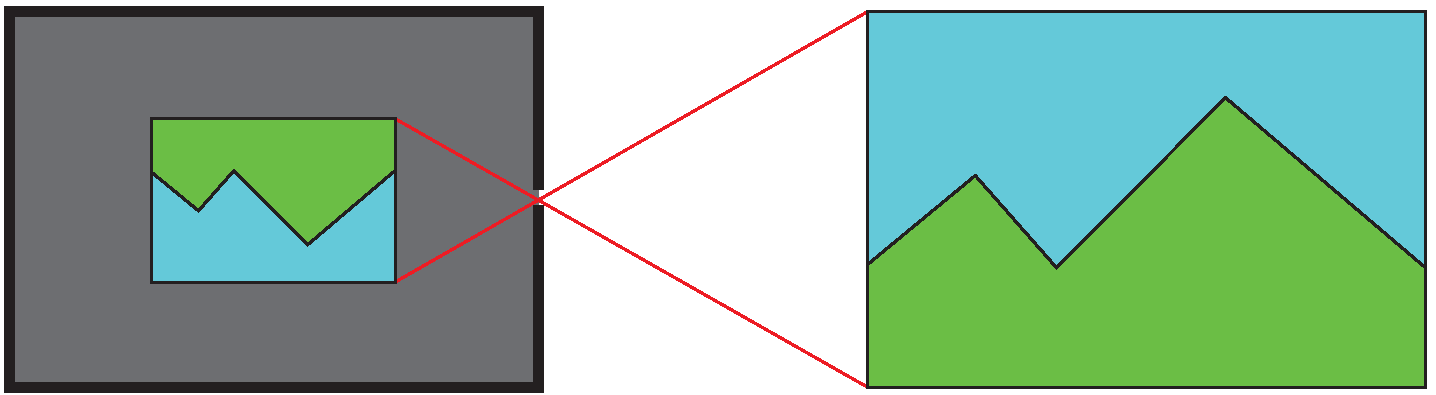
\includegraphics[width=\textwidth]{images/camera oscura.pdf}
\end{figure}

Con questa configurazione l'immagine risulta riflessa rispetto al mondo esterno.
Utilizziamo quindi un ulteriore astrazione, in cui poniamo il sensore al di fuori della camera, mantenendo però la condizione in cui la luce deve passare per l'apertura puntiforme per essere catturato nell'immagine (figura \ref{fig:camera model}).
È facilmente verificabile che l'immagine così ottenuta sia uguale all'immagine precedente ma riflessa, e quindi sia coerente con la realtà.
\begin{figure}
    \caption{Sensore esterno alla camera}
    \label{fig:camera model}
    \centering
    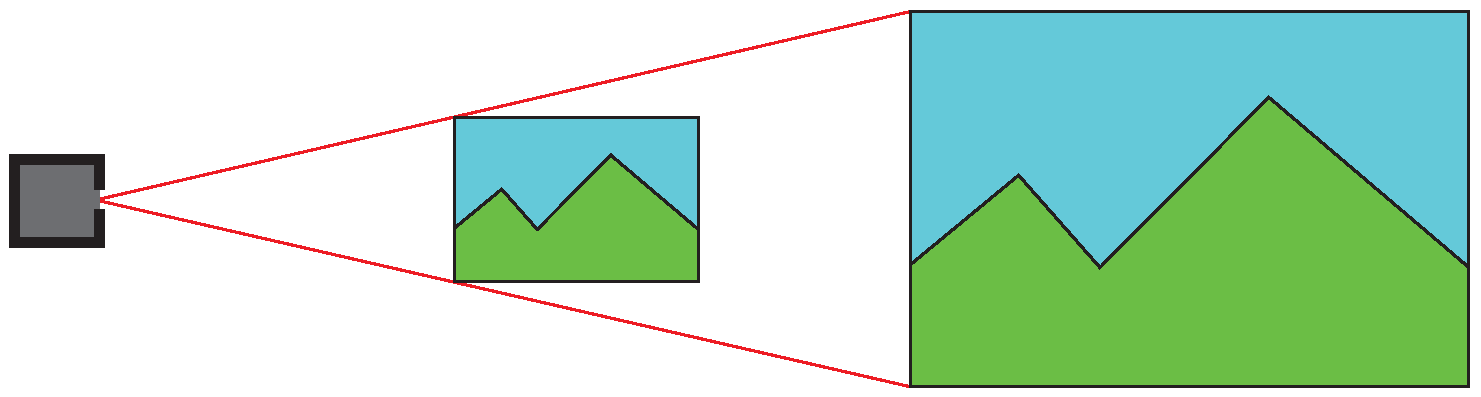
\includegraphics[width=\textwidth]{images/camera astratta.pdf}
\end{figure}

Ciò a cui siamo interessati non è però generare l'immagine, ma conoscere la configurazione dello spazio reale con cui l'immagine è stata generata.
Dato che l'immagine è generata da raggi di luce che si muovono in linea retta possiamo affermare che ad ogni punto $P'$ dell'immagine corrisponde un punto $P$ nello spazio reale e che questo punto si trova sulla linea che passa per la camera e $P'$.
Questo non è abbastanza per individuare $P$, in quanto una linea contiene infiniti punti.
Possiamo risolvere questo problema conoscendo il contesto che stiamo provando a correggere.
Dato che questo contesto è il contesto stradale, possiamo supporre che le entità a cui siamo interessati siano poggiate sulla strada, che approssimiamo con un piano bidimensionale.
Il punto $P$ è quindi contenuto sia nel raggio di luce che nel piano stradale.
Assegnamo delle coordinate ai vari elementi per calcolare la trasformazione (figura \ref{fig:camera coords}).
\begin{figure}
    \caption{Modello con coordinate}
    \label{fig:camera coords}
    \centering
    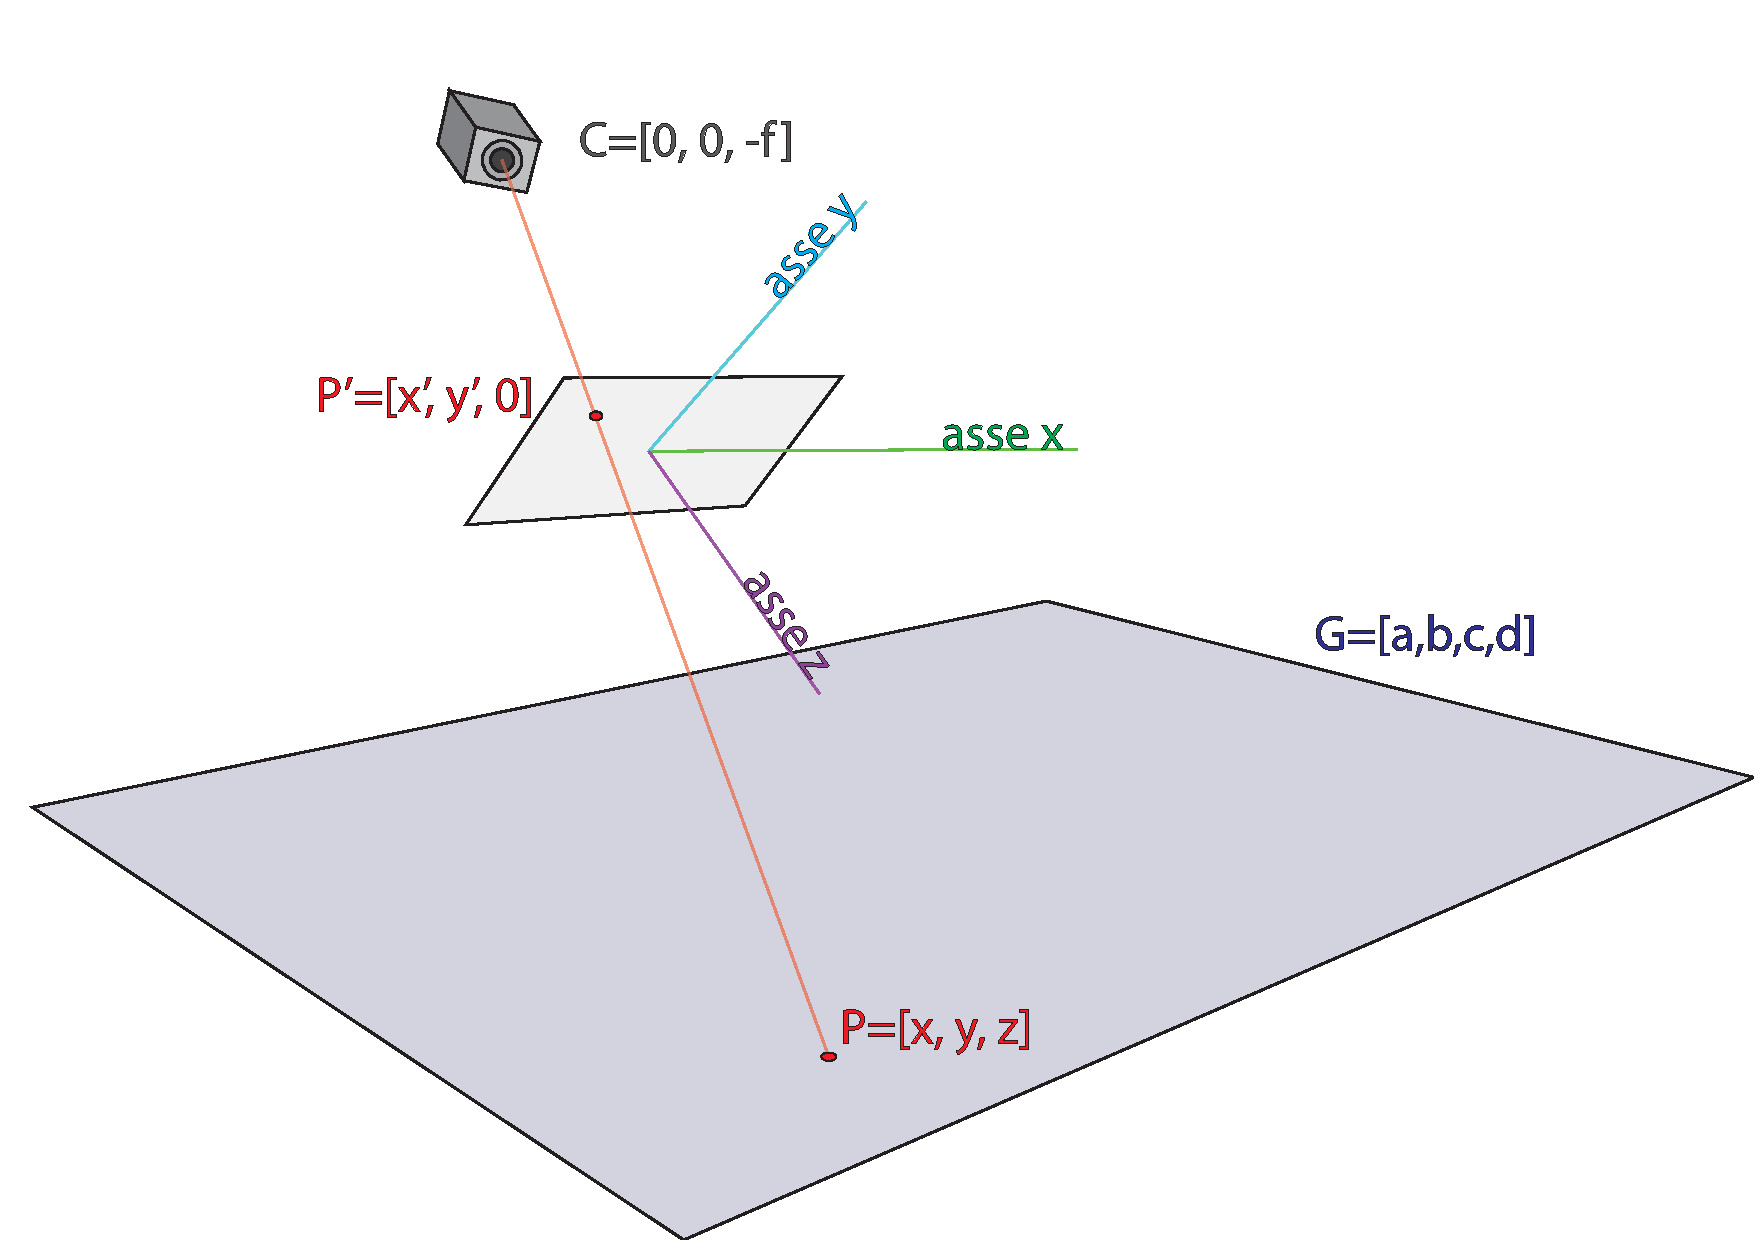
\includegraphics[width=\textwidth]{images/camera coords.pdf}
\end{figure}

Possiamo ricavare il punto $P$ trovando l'intersezione tra il piano $G$ e la linea $\overline{CP'}$.
In $R^3$ una linea è identificata da un sistema di 2 equazioni.
Il punto $P$ è quindi definito dal sistema di 3 equazioni in \ref{eq:system}.
\begin{equation}
    \label{eq:system}
    P = 
    \left\{
    \begin{aligned}
         & ax + bx + cz + d = 0                       \\
         & \frac{1}{x'}x - \frac{1}{y'}y + 0z + 0 = 0 \\
         & 0x -  \frac{1}{y'}y + \frac{1}{f}z + 1 = 0 \\
    \end{aligned}
    \right.
\end{equation}

Risolvendo il sistema in \ref{eq:system} troviamo le equazioni in \ref{eq:cartesian}.
\begin{equation}
    \label{eq:cartesian}
    \begin{aligned}
         & x = \left( \frac{cf - d}{ax' + by' + cf} \right) x'    \\
         & y = \left( \frac{cf - d}{ax' + by' + cf} \right) y'    \\
         & z = \left( \frac{cf - d}{ax' + by' + cf} - 1 \right) f \\
    \end{aligned}
\end{equation}
Le equazioni così trovate non sono lineari.
Possiamo però definire una nuova coordinata $\lambda$ e trasformare le equazioni in \ref{eq:cartesian} nelle equazioni in \ref{eq:homogeneous}.
\begin{equation}
    \label{eq:homogeneous}
    \begin{aligned}
        \lambda x & = (cf - d) x'       \\
        \lambda y & = (cf - d) y'       \\
        \lambda z & = -fax' - fby' - fd \\
        \lambda   & = ax' + by' + cf    \\
    \end{aligned}
\end{equation}

Le coordinate $[\lambda x, \lambda y, \lambda z, \lambda]^T$ sono chiamate \emph{coordinate proiettive omogenee}.
La forma normale $N$ di un vettore $V$ definito in \emph{coordinate proiettive omogenee} si ottiene attraverso la formula $N = \displaystyle\frac{V}{\lambda_V}$.
$N$ è quindi della forma $N = [x, y, z, 1]^T$.
È perciò semplice la conversione da \emph{coordinate cartesiane} a \emph{coordinate proiettive} e viceversa.
Possiamo quindi definire le equazioni trovate come trasformazione lineare in coordinate proiettive.
La matrice relativa a questa trasformazione è in \ref{eq:projmat}.
\begin{equation}
    \label{eq:projmat}
    J_{(f, [a, b, c, d])} =
    \begin{bmatrix}
        cf - d & 0      & 0   \\
        0      & cf - d & 0   \\
        -fa    & -fb    & -fd \\
        a      & b      & cf  \\
    \end{bmatrix}
\end{equation}
Questo sistema di coordinate è lo stesso utilizzato per applicare le classiche trasformazioni lineari di traslazione, rotazione, scala e shear.
Tutte queste trasformazioni rimangono quindi applicabili anche dopo il cambio di coordinate e possono essere combinate con la trasformazione di proiezione $J$ trovata.

Riassumiamo i passaggi da compiere in modo da comporre la trasformazione $M$ completa:
\begin{enumerate}
    \item Cambiare coordinate da $R^2$ omogeneo in $R^3$ omogeneo, settando $z=0$.
    \item Scalare l'immagine, rendendo $h = 1, w = w/h$.
    \item Riflettere l'asse Y dell'immagine, in modo che incrementi muovendosi verso l'alto.
    \item Traslare l'origine dell'immagine al centro di questa.
    \item Proiettare l'immagine sul piano $G$, calcolando e applicando $J$.
    \item Applicare l'inversa della trasformazione dell'immagine, così da avere $z=0$ per tutti i punti ottenuti.
    \item Rimuovere la coordinata $z$, così da tornare in $R^2$ omogeneo.
\end{enumerate}
Per calcolare il piano $G$, necessario per calcolare $J_{(f, G)}$, si deve:
\begin{enumerate}
    \item Applicare al piano $[0, 0, 1, 0]$, che è il piano in cui $z=0$, l'inversa della rotazione dell'immagine.
    \item Calcolare l'origine del piano $O$, applicando l'inversa della trasformazione dell'immagine al punto $[0, 0, 0, 1]$.
    \item Applicare al piano la ``traslazione per piani'' che porta l'origine nel punto calcolato in precedenza. Questa ``traslazione per piani'' è uguale alla trasposta dell'inversa della traslazione per punti.
\end{enumerate}
Quindi abbiamo, indicando come $I$ la trasformazione completa dell'immagine, $I_R, I_T$ rispettivamente rotazione e traslazione dell'immagine, $T_{(x, y, z)}$ la traslazione che porta $[0, 0, 0, 1]$ in $[x, y, z, 1]$, $S_{(x, y, z)}$ la scala che porta $[1, 1, 1, 1]$ in $[x, y, z, 1]$:
\begin{equation}
    \begin{aligned}
        O & = I^{-1} \cdot [0, 0, 0, 1]                       \\
        G & = T_{(O)}^{-1T} \cdot I_R^{-1} \cdot [0, 0, 1, 0] \\
        M & =
        \begin{bsmallmatrix}
            1 & 0 & 0 & 0 \\
            0 & 1 & 0 & 0 \\
            0 & 0 & 0 & 1 \\
        \end{bsmallmatrix}
        \cdot I^{-1} \cdot J_{(f, G)} \cdot T_{(0.5, w/2h)} \cdot S_{(1/h, -1/h, 1)} \cdot
        \begin{bsmallmatrix}
            1 & 0 & 0 \\
            0 & 1 & 0 \\
            0 & 0 & 0 \\
            0 & 0 & 1 \\
        \end{bsmallmatrix}                                   \\
    \end{aligned}
\end{equation}
La matrice $M$ trovata è una matrice $3x3$.
È perciò una matrice omografica in $R^2$ omogeneo.
Il punto $P = M \cdot P'$ deve perciò essere normalizzato e convertito in coordinate cartesiane prima di essere utilizzato dal resto del sistema.

\chapter{Funzionalità}
\label{sec:funzionalita}

% TODO: METTI IMMAGINI
\section{Modulo di correzione}
Il sistema in cui il modulo di correzione è inserito si occupa di individuare, classificare e tracciare le entità presenti nello stream video ricavato dalla camera.
Con i dati ottenuti effettua poi, attraverso l'utilizzo di euristiche sperimentali, la rilevazione di anomalie.
Le anomalie trattate sono:
% TODO: standardizza
\begin{itemize}
    \item Cambio di corsia non permesso
    \item Traffico congestionato
    \item Attraversamento pedonale fuori dalle strisce 
    \item Veicolo al di fuori della strada (es. marciapiede) %ew
    \item Urto tra veicoli e tra veicolo e pedone
    \item Sosta non consentita
\end{itemize}
La corretta implementazione del modulo di correzione, che è posto come filtro tra la classificazione e il tracciamento delle entità, ha il fine di migliorare i risultati della rilevazione delle anomalie elencate sopra.

\begin{figure}
    \caption{Sistema di rilevazione di anomalie in funzione}
    \label{fig:anomalie}
    \centering
    
\includegraphics[width=.66\textwidth]{images/placeholder.png}
\end{figure}

\section{Strumento interattivo}
Lo strumento interattivo è sviluppato sulla base dell'ipotesi che l'operatore umano sia in grado di riconoscere un'immagine in cui non è presente la \emph{distorsione prospettica}, in quanto questa assomiglia a una ``vista dall'alto'', in cui le linee parallele e perpendicolari nella realtà appaiono parallele e perpendicolari. 
Linee disposte in questo modo sono comuni nell'ambito stradale.
Lo strumento fornisce quindi la possibilità di manipolare i parametri di \emph{lunghezza focale}, \emph{distanza tra piano e immagine (altezza)}, \emph{rotazione sull'asse x}, \emph{rotazione sull'asse y}.
Il primo è controllato attraverso la \emph{rotellina del mouse}, gli altri due con \emph{click \& drag} sull'immagine.
La \emph{rotazione sull'asse z} è raramente necessaria in situazioni reali e non è quindi manipolabile.

Lo strumento mostra una porzione dell'immagine dopo che la trasformazione è stata applicata.
L'operatore è quindi in grado di valutare la bontà della trasformazione visivamente.
Dato che la trasformazione non mantiene forma e dimensioni dell'immagine non è possibile applicare la trasformazione all'immagine e poi mostrarla.
Lo strumento quindi parte dalle coordinate dell'immagine già manipolata e per ogni pixel applica la trasformazione inversa.
Con le coordinate trovate va a copiare il pixel dell'immagine originale nella posizione trovata.
La trasformazione utilizzata per la manipolazione ha inoltre delle modifiche rispetto a quella indicata nel capitolo \ref{sec:teoria}: l'altezza utilizzata è fissata a 0 e la trasformazione viene traslata in modo da mantenere il punto centrale dell'immagine nella stessa posizione prima e dopo la trasformazione.
Senza queste modifiche la manipolazione dell'immagine risulta disorientante e difficile.

Sono presenti i controlli di navigazione relativi a \emph{zoom}, \emph{posizione x}, \emph{posizione y}.
Tutti i parametri, compresi quelli relativi a \emph{lunghezza focale} e \emph{rotazione}, sono modificabili con bottoni e campi testuali.
Una volta manipolata correttamente l'immagine è possibile salvare la matrice di trasformazione e i parametri configurati.
La matrice salvata, a differenza di quella della manipolazione, è generata usando anche \emph{l'altezza}.
Anche questa è traslata per mantenere il punto centrale dell'immagine originale nella stessa posizione.

Per migliorare i risultati è stato fornito un bottone che permette di visualizzare l'immagine originale.
È stata aggiunta anche una modalità di misurazione che permette di inserire segmenti che indicano la loro dimensione dopo la trasformazione.
Questi segmenti vengono manipolati visivamente insieme all'immagine ma le misure sono relative alla trasformazione che verrà poi salvata.

\begin{figure}
    \caption{Stumento interattivo: interfaccia}
    \label{fig:tool view}
    \centering
    
\includegraphics[width=.66\textwidth]{images/placeholder.png}
\end{figure}

\begin{figure}
    \caption{Stumento interattivo: modalità di misurazione}
    \label{fig:tool measure}
    \centering
    
\includegraphics[width=.66\textwidth]{images/placeholder.png}
\end{figure}

\chapter{Architettura e implementazione}
\label{sec:implementazione}

% TODO: AGGIUNGI IMMAGINI, RIFERIMENTI 

% Definire e desccrivere nei dettagli l'architettura a blocchi, descrivendo ciascun blocco e i collegamenti.
% Non è ancora necessario dare dettagli implementativi, che andranno nel capitolo dedicato.
% Descrizione tecnologie utilizzate per implementare ciascun blocco.
% Qui vanno i dettagli implementativi per ciascun blocco dell'architettura definita nel capitolo precedente.
% Potrebbe convenire replicare l'immagine dell'architettura, definendo all'interno dell'immagine dettagli implementativi come ad esempio i nomi dei moduli utilizzati e le tecnologie utilizzate per implementarli.

\section{Sistema di rilevazione anomalie}
Il sistema di rilevazione anomalie, in cui il modulo di correzione è implementato, è costituito dai moduli in figura \ref{fig:sys modules}.
\begin{figure}
    \caption{Architettura del sistema di rilevazione anomalie}
    \label{fig:sys modules}
    \centering
    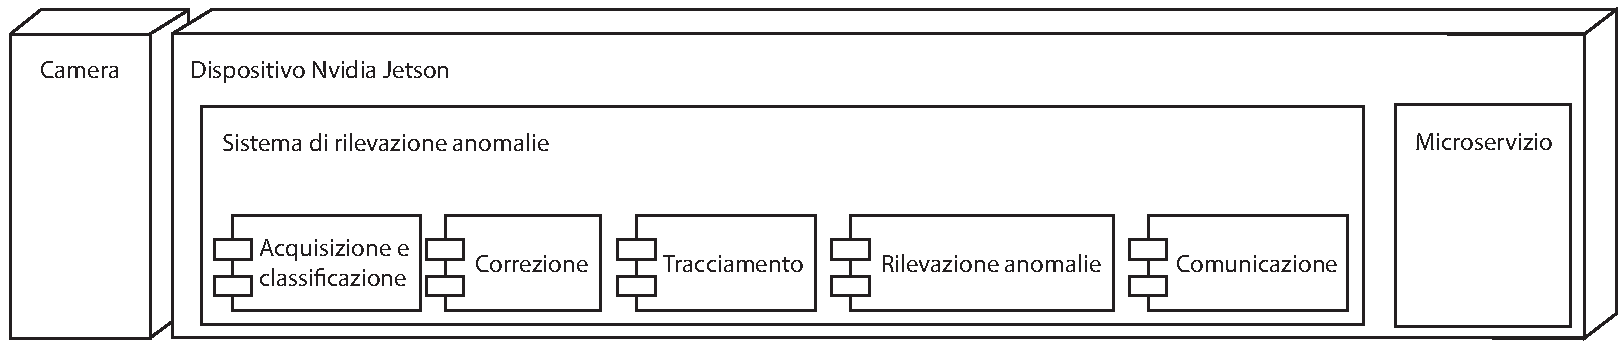
\includegraphics[width=\textwidth]{images/arch.pdf}
\end{figure}
Il sistema è implementato sul dispositivo \emph{Nvidia Jetson Xaxier}\cite{arch:jetson} ed è sviluppato su \emph{Ubuntu 18.04}\cite{arch:ubuntu}.
Il linguaggio di sviluppo è \emph{Python 3.6}\cite{arch:python}.
Per la gestione delle operazione di algebra lineare sono stati utilizzati i package \emph{Numpy}\cite{arch:numpy} e \emph{SciPy}\cite{arch:scipy}.
La pipeline di acquisizione è gestita dalla libreria \emph{GStreamer}\cite{arch:gstreamer}.
La classificazione è effettuata dal modulo di inferenza fornito dall'\emph{SDK Nvidia Deepstream}\cite{arch:deepstream}.
Questo modulo di inferenza è configurato per il modello di \emph{Object Detection YoloV4}\cite{arch:yolo}.

Il modulo di correzione si occupa della rimozione di duplicati ed occlusioni e della correzione della distorsione prospettica descritta in questa tesi.

Il modulo di tracking effettua il tracciamento delle entità, utilizzando una funzione di smoothing per ridurre le imprecisioni della classificazione.
Il tracking è effettuato sia utilizzando l'ultima posizione conosciuta, sia la posizione predetta in base a velocità e accelerazione.

Il modulo di rilevazione di anomalie si occupa di posizionare le entità all'interno della mappa stradale (preconfigurata da un operatore), di assegnarvi una forma approssimata e di comunicare con i sottomoduli di rilevazione delle singole anomalie.
I dati relativi alla mappa sono gestiti attraverso coordinate baricentriche e sono utilizzati per \emph{Cambio di corsia}, \emph{Sosta vietata}, \emph{Persona in strada}, \emph{Invasione di area}.
Gli \emph{Urti} sono verificati simulando la posizione futura delle entità e cercando intersezioni con l'algoritmo \emph{GJK}\cite{arch:gjk}.

Il modulo di comunicazione ottiene i dati relativi alle anomalie e lo stream video e si occupa di salvare segmenti di video in cui sono presenti una o più anomalie.
I dati relativi alle anomalie e il percorso del video sono inviati tramite richiesta HTTP al \emph{Microservizio}, implementato nello stesso dispositivo, che gestisce la comunicazione col backend principale.
Il modulo di comunicazione utilizza \emph{OpenCV}\cite{arch:opencv} per il salvataggio del video e \emph{Requests}\cite{arch:requests} per la comunicazione HTTP.
Il \emph{Microservizio} è implementato con \emph{NodeJS}\cite{arch:nodejs}, \emph{Express}\cite{arch:express}, \emph{Sequelize}\cite{arch:sequelize} e utilizza un database \emph{MySQL}\cite{arch:mysql}.

\section{Strumento interattivo}
Lo strumento interattivo è scritto in \emph{TypeScript}\cite{arch:typescript} e utilizza il framework \emph{SvelteKit}\cite{arch:sveltekit}.
Per le operazioni di algebra lineare è utilizzato \emph{MathJS}\cite{arch:mathjs}.
Per implementare il rendering dell'immagine manipolata è stato utilizzato \emph{GpuJS}\cite{arch:gpujs}, in quanto ha consentito di evitare i costi di tempo richiesti per imparare \emph{WebGL}\cite{arch:webgl}.
Questa libreria non è però abbastanza matura e presenta alcuni comportamenti non ideali, ed è quindi raccomandabile spendere il tempo necessario per imparare \emph{WebGL} in futuro.
Tutto il resto delle funzionalità è implementato attraverso l'uso di \emph{WebAPI}\cite{arch:webapi} e \emph{Svelte}\cite{arch:svelte}.
Il deploy è effettuato come \emph{SPA}\cite{arch:spa} su \emph{GitHub Pages}\cite{arch:ghpages}.

\chapter{Testing}
\label{sec:testing}
Come è stato validato il sistema

\section{Sottosezione testing}
\label{sec:nomesottosezione2}


\subsection{Sottosottosezione testing}
\label{sec:nomesottosottosezione}


\chapter{Conclusioni}
\label{sec:conclusioni}

L'obiettivo iniziale di correggere la \emph{distorsione prospettica} presente nelle misure di posizione e velocità è stato perciò raggiunto.
Questo risultato è stato ottenuto modellando il problema matematicamente in modo da comprendere la natura della distorsione e da individuare le approssimazioni necessarie alla sua risoluzione.
La fase complicata si è rivelata essere la generazione della trasformazione correttiva e non la sua applicazione.
È stato perciò necessario sviluppare uno strumento esterno interattivo con cui semplificare tale generazione.
Il lavoro fatto è stato poi validato confrontando i risultati ottenuti dal sistema di rilevazione di anomalie prima e dopo l'implementazione della soluzione proposta.

Possibili sviluppi futuri della soluzione trovata sono il permettere la definizione di trasformazioni sulla stessa immagine, in modo da gestire ambienti in cui un singolo piano non rende un'approssimazione soddisfacente.
Inoltre potrebbe essere interessante implementare i metodi discussi nella sezione riguardante lo stato dell'arte (Capitolo \ref{sec:introduzione}) nello strumento interattivo, come supporto all'operatore.

% NON SUDDIVISA per punti ma discorsiva (io suddivido per punti per chiarezza):
% •	l'obiettivo era (notare il tempo al passato) bl bla ripeti quanto detto in cap 1
% •	Abbiamo perseguito gli scopi preposti facendo bla bla ribadisci quanto raccontato nella tesi
% •	I risultati sono bla bla (sottolinea le cose + salienti
% •	commenti, limiti del lavoro, considerazioni, conclusioni e sviluppi futuri.


\pagestyle{empty}

\chapter*{Ringraziamenti}
Ringrazio Salvatore, Silvio e Sebastian che mi hanno fatto trovare questo template pronto.


\addcontentsline{toc}{chapter}{Ringraziamenti}%

\bibliographystyle{splncs04}
\bibliography{bibliography}

\nocite{*}



% ----------------- ELENCO DELLE FIGURE/TABELLE ------------------------
\cleardoublepage
\listoffigures
\listoftables

\cleardoublepage


\end{document}
